\chapter{Design Milestone \\
  \small{\textit{-- Evan Ciok, Sophia DiCuffa, Carson McManus}}
  \index{Chapter!designMilestone}
  \index{Design Milestone}
  \label{Chapter::designMilestone}}

% Add a section and label it so that we can reference it later
\section{Desgin Milestone \label{Section::designMilestone}}

\subsection{Problem Statement}
Problem Statement

This project aims to model and overhaul the architecture of OpenTogetherTube, a platform for watching videos with 
friends. The current OTT system runs on node.js, which runs JavScript code in a single thread. An event loop exists 
with the function of handling incoming requests, but this can get backed up as the number of clients to handle 
increases. This leads to response times that can be far higher than desired for a responsive platform like OTT.
A vertical or horizontal approach can be taken in an effort to alleviate the overbearing load. Vertical scaling 
of the system to make it more network efficient would be effective, but there is an imposed ceiling on its impact.
Horizontal scaling on the other hand has no such ceiling. By introducing more instances of the backend via 
node.js on new processing units the load can be distributed and handled much more efficiently. This architectural
remodel would allow OTT to gain the capacity for large scale expansion moving forward.  

Tagline: Horizontal Scaling for OpenTogetherTube

\subsection{Project Description}
Project Description

OpenTogetherTube is a very complex piece of software, and we want to be prepared to scale up when the time comes. OTT's current architecture is haphazardly planned and pretty inefficient. 
Horizontal scaling is taking what is on one computer and putting it on another computer as well. Adding multiple computers can spread the load across multiple devices.

OTT is pretty network efficient, so network throughput is not a huge concern. Modern OSes can handle tons and tons of TCP connections to a single port. However, a more pressing concern is that each user that joins a room puts more load on the Node.js event loop.
It needs to be possible to spin up and take down nodes on demand.

\subsection{Use Cases}



\subsection{Design Sketches}
Design Sketches

There are four sequence flows to display our design in action. First, there is joining a room (Figure \ref{Figure::room}). Next, there is joining an unloaded room (Figure \ref{Figure::unloaded}). Then, there is generating and joining a temporary room (Figure \ref{Figure::temp}). Last, we have creating and joining a new named temporary room, our edge case (Figure \ref{Figure::edge}).

\begin{figure}
  \centering
  \scalebox{0.6}{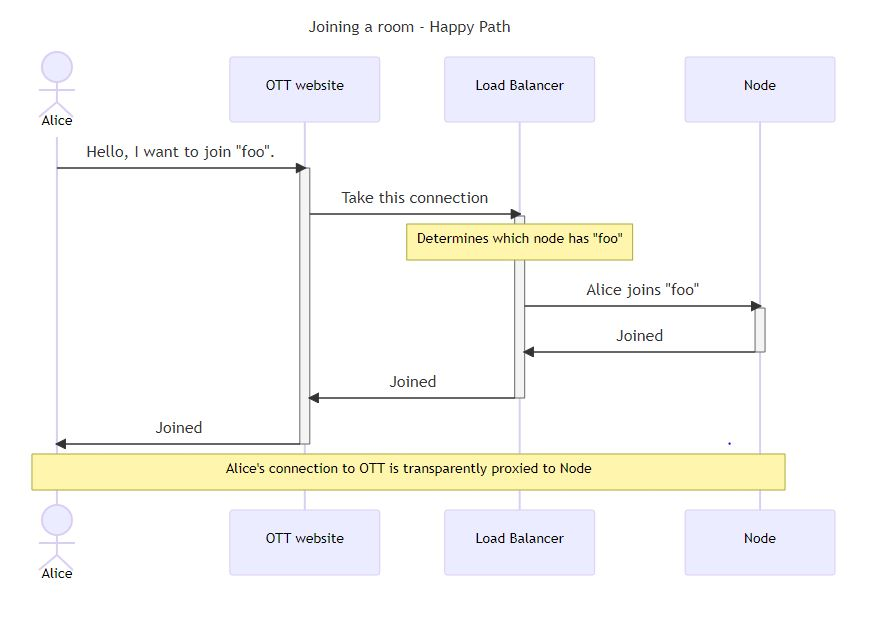
\includegraphics{Figures/designMilestone/room.jpg}}
  \caption{\label{Figure::room} Joining a room.}
\end{figure}

\begin{figure}
  \centering
  \scalebox{0.7}{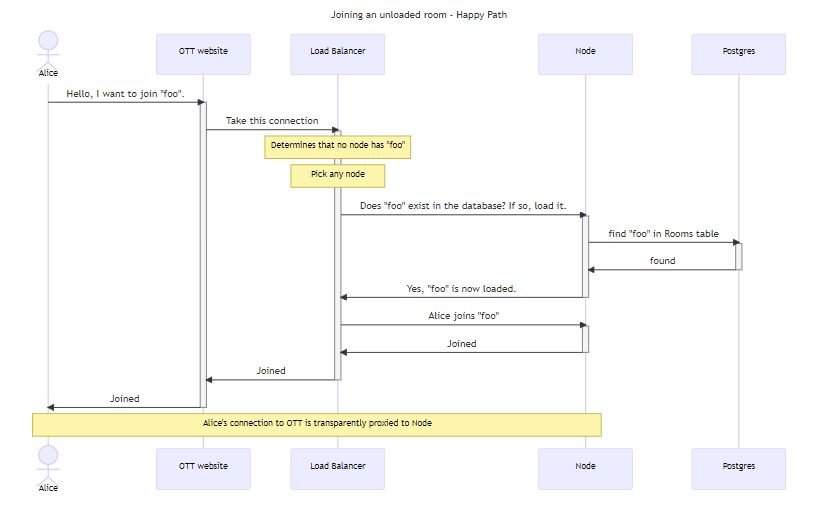
\includegraphics{Figures/designMilestone/unloaded.jpg}}
  \caption{\label{Figure::unloaded} Joining an unloaded room.}
\end{figure}

\begin{figure}
  \centering
  \scalebox{0.7}{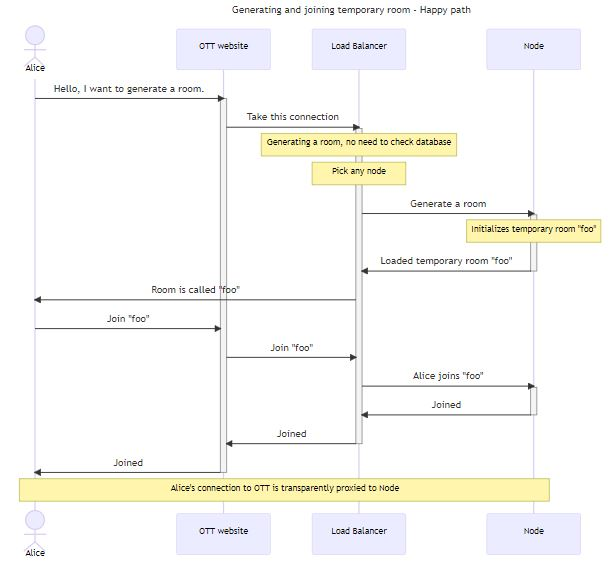
\includegraphics{Figures/designMilestone/temp.jpg}}
  \caption{\label{Figure::temp} Generating and joining a temporary room.}
\end{figure}

\begin{figure}
  \centering
  \scalebox{0.7}{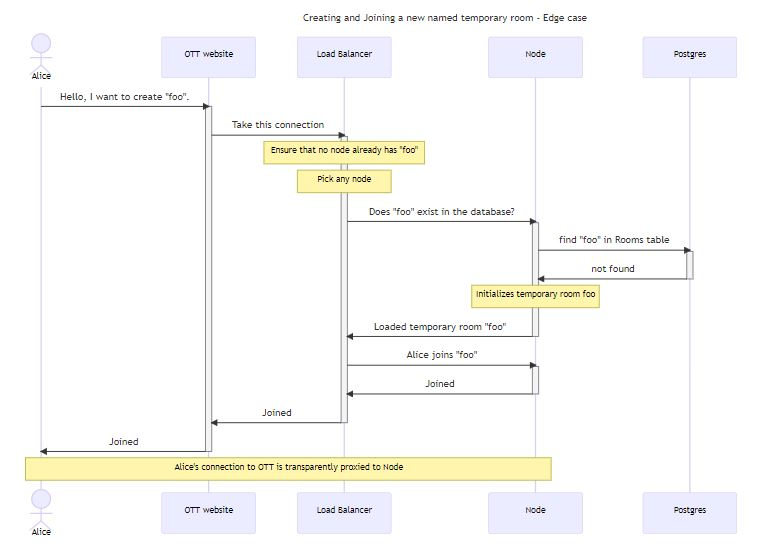
\includegraphics{Figures/designMilestone/edge.jpg}}
  \caption{\label{Figure::edge} Generating and joining a new named temporary room.}
\end{figure}


\newpage

\subsection{Architecture Design}
Architecture Design

In our configuration, the node containing the loaded room would receive the client's connections through a proxy (Figure \ref{Figure::architecture}). This relieves all nodes from the responsibility of checking for temporary rooms as it is now delegated to the load balancers. As a result, the load balancers handle the task of managing temporary rooms, freeing up the nodes to focus on other responsibilities.

\begin{figure}
  \centering
  \scalebox{0.5}{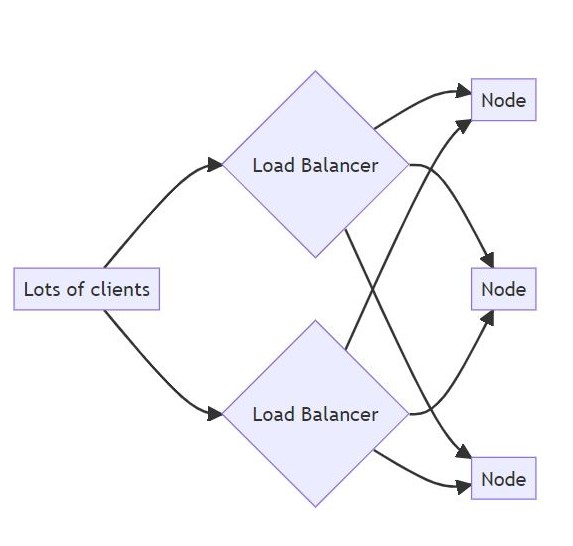
\includegraphics{Figures/designMilestone/Architecture.jpg}}
  \caption{\label{Figure::architecture} Architecture Design diagram.}
\end{figure}

